% Auto-generated figure include snippets.
\begin{figure*}[t]
  \centering
  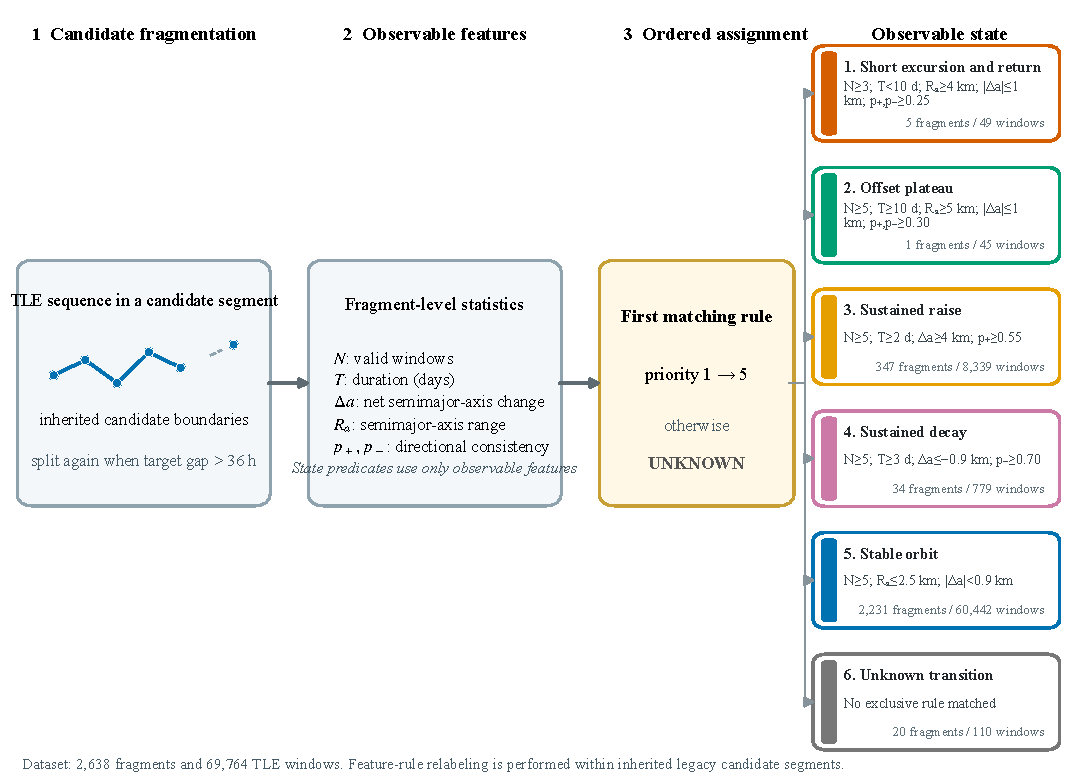
\includegraphics[width=\textwidth]{figures/tle_state_use_case/fig1_observable_state_definition.pdf}
  \caption{Observable-state feature-rule relabeling workflow. Candidate boundaries are inherited from the prior rule pipeline and additionally split at target gaps longer than 36 h. Within each candidate, the state label uses only observable fragment statistics and the first satisfied predicate in the ordered rule set. Thus this is feature-only relabeling within inherited candidates, not an intent-free segmentation pipeline. Counts cover the full train+validation+test v2 label set.}
  \label{fig:tle-state-definition}
\end{figure*}

\begin{figure*}[t]
  \centering
  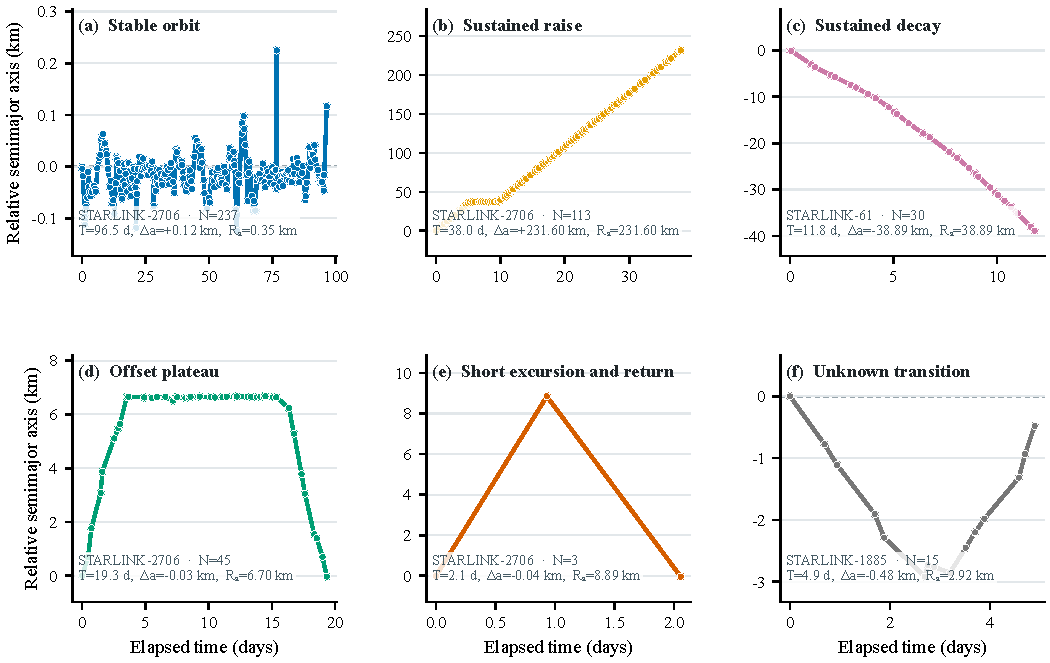
\includegraphics[width=\textwidth]{figures/tle_state_use_case/fig2_observable_state_examples.pdf}
  \caption{Illustrative, hand-selected TLE-observable fragments. Each panel shows semimajor-axis change relative to the fragment start against true elapsed time; panel axes are independently scaled. Panels show (a) stable orbit, (b) sustained raise, (c) sustained decay, (d) offset plateau, (e) short excursion and return, and (f) unknown transition. Four panels use STARLINK-2706; only one offset-plateau and five short-excursion fragments exist, so those panels are qualitative cases rather than population summaries.}
  \label{fig:tle-state-examples}
\end{figure*}

\begin{figure*}[t]
  \centering
  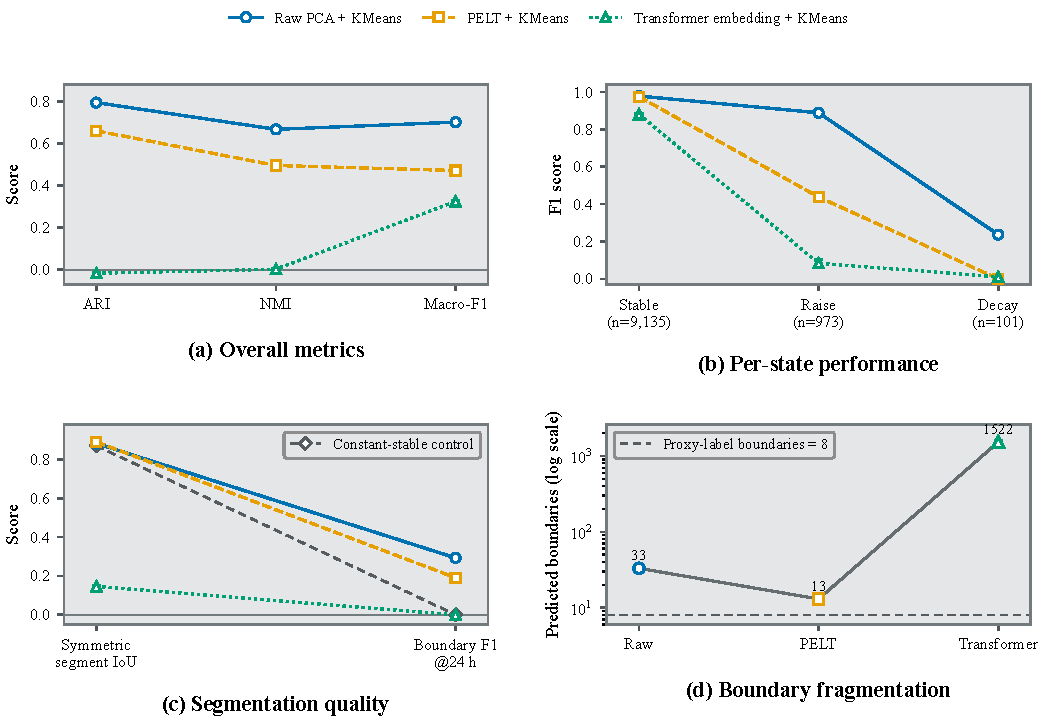
\includegraphics[width=\textwidth]{figures/tle_state_use_case/fig3_method_comparison.pdf}
  \caption{Retrospective $K=3$ comparison on the stable, sustained-raise, and sustained-decay TLE-observable proxy classes. Cluster-to-class Hungarian mappings use training labels only. Panels report (a) clustering and mapped classification scores, (b) per-state F1 and support, (c) symmetric segment IoU and boundary F1 with gray diamonds for the constant-stable control, and (d) predicted boundary counts. Bars show mean $\pm$ standard deviation over seeds 42--44 on the same retrospective 10,209-window, 376-target slice. Decay has 101 windows and only eight proxy-label boundaries exist. Segment IoU is strongly stable-class dominated; the labels describe observable trajectory shape, not operational intent.}
  \label{fig:tle-method-comparison}
\end{figure*}

% Auto-generated by gen_results_table.py; requires booktabs.
\begin{table*}[t]
\centering
\caption{Retrospective $K=3$ clustering performance on the three quantitative TLE-observable proxy classes. Cluster-to-class Hungarian mappings use training labels only. All methods use the same 10,209-window, 376-target test slice; decay has 101 windows and boundary scores use only eight proxy-label boundaries. Learned-method values are mean $\pm$ standard deviation over three seeds. The labels describe observable shape, not operational intent.}
\label{tab:tle-observable-clustering}
\footnotesize
\setlength{\tabcolsep}{3.2pt}
\begin{tabular}{lrrrrrr}
\toprule
Method & ARI & NMI & Macro-F1 & Sym. segment IoU & Boundary-F1@24h & Pred. boundaries \\
\midrule
Constant stable (control) & 0.000 & 0.000 & 0.315 & 0.871 & 0.000 & 0 \\
Raw + KMeans & \textbf{0.794 $\pm$ 0.000} & \textbf{0.667 $\pm$ 0.001} & \textbf{0.701 $\pm$ 0.000} & 0.883 $\pm$ 0.000 & \textbf{0.293 $\pm$ 0.000} & 33.0 $\pm$ 0.0 \\
PELT + KMeans & 0.660 $\pm$ 0.000 & 0.495 $\pm$ 0.000 & 0.471 $\pm$ 0.000 & \textbf{0.891 $\pm$ 0.000} & 0.190 $\pm$ 0.000 & 13.0 $\pm$ 0.0 \\
Transformer + KMeans & -0.017 $\pm$ 0.004 & 0.003 $\pm$ 0.002 & 0.324 $\pm$ 0.004 & 0.146 $\pm$ 0.005 & 0.000 $\pm$ 0.000 & 1522.3 $\pm$ 52.3 \\
\bottomrule
\end{tabular}
\vspace{2pt}
\parbox{0.98\textwidth}{\footnotesize The test slice contains 10,209 primary-state windows from 376 NORAD targets and 8 proxy-label boundaries. The deterministic constant-stable control attains 0.8705 segment IoU, showing this metric's sensitivity to the 9,135 stable windows.}
\end{table*}

